\documentclass[conference,letterpaper,10pt]{IEEEtran}
\IEEEoverridecommandlockouts

\usepackage{cite}
\usepackage{amsmath,amssymb,amsfonts}
\usepackage{graphicx}
\usepackage{booktabs}
\usepackage{array}
\usepackage{xcolor}
\usepackage{textcomp}
\usepackage{caption}
\captionsetup{font=small,labelfont=bf}

% --- Placeholder box for figures you will insert later -----------------------
\newcommand{\imgph}[2]{%
  \fbox{\parbox[c][#1][c]{0.95\linewidth}{\centering\small\itshape #2}}%
}
% ---------------------------------------------------------------------------

\begin{document}

\title{Semantic-Guided Manipulation for Targeted Object Retrieval in Highly Cluttered Environments\\
{\large Progress Report}}

\author{
    \IEEEauthorblockN{Mahyar Fardinfar}
    \IEEEauthorblockA{mahyar.fardinfar@bilkent.edu.tr}
    \and
    \IEEEauthorblockN{Salman Awan}
    \IEEEauthorblockA{s.awan@bilkent.edu.tr}
    \and
    \IEEEauthorblockN{Hakan Muluk}
    \IEEEauthorblockA{hakan.muluk@bilkent.edu.tr}
    \and
    \IEEEauthorblockN{Pinar Gul}
    \IEEEauthorblockA{pinar.gul@bilkent.edu.tr}
    \and
    \IEEEauthorblockN{Osama Awad}
    \IEEEauthorblockA{saed.awad@bilkent.edu.tr}
}

\maketitle

\section{Point-cloud construction}

This section describes our segmentation pipeline, which operates in two
stages. The first stage performs instance segmentation directly on the
volumetric (voxel) reconstruction in the absence of texture information.
The second stage performs language-guided semantic segmentation on
rendered RGB views of a multi-object scene, returning the mask of a
single queried object that is later back-projected to obtain the
corresponding point cloud.

\subsection{Instance Segmentation on 3D Voxel Data}
\label{subsec:instance}

In the first stage, the only available input was the voxelized
reconstruction of the scene (Fig.~\ref{fig:envs}a); per-voxel RGB
information was either unavailable or unreliable because of the
rendering pipeline. We evaluated three candidate approaches for
separating the voxel grid into distinct object instances.

\textbf{Color-based segmentation.} We first projected the surface voxels
back onto image space and applied classical color-space clustering. This
method was computationally light but failed to yield clean object
boundaries: the directional lighting of the simulation environment cast
strong shadows on otherwise uniform surfaces, which caused single
objects to be split into multiple regions. Moreover, this algorithm could not identify two adjacent objects with same color.

\textbf{SAM2.} We next evaluated SAM2~\cite{sam2}, which produced
substantially cleaner mask boundaries. However, SAM2 is class-agnostic (which was good for our task at this stage) but it failed to identify all the objects because our object domain was not, obviously, in its training data domain. Hence it does not process text queries it was also impossible to add context to it about the dynamics of our environment (simulation of voxels). To overcome this problem, We have tried integrating Dinov2~\cite{dinov2} with SAM2 which produced fairly good results but still lacked in detection of all the objects in the scene. 

\textbf{SAM3.} Finally, we evaluated SAM3~\cite{sam3}, which extends the
SAM family with native text prompting. SAM3 retained the boundary
quality of SAM2 while also enabling language-guided retrieval of a
specific instance from the rendered voxel view, which removed the need
for a separate language embedding module. This achieved the best result for our experiment among all the tested methods.

\begin{figure}[!t]
\centering
\begin{minipage}[t]{0.48\columnwidth}
  \centering
\includegraphics[width=\linewidth]{voxel_env.png}\\[2pt]  
{\footnotesize (a) Voxel environment}
\end{minipage}\hfill
\begin{minipage}[t]{0.48\columnwidth}
  \centering
\includegraphics[width=\linewidth]{new_env.png}\\[2pt]  
  {\footnotesize (b) Random-object environment}
\end{minipage}
\caption{Sample views of the two simulation environments used in this
work. (a) Voxel-only scene used to evaluate instance segmentation
(Sec.~\ref{subsec:instance}); (b) Multi-color scene with
several distinctly-coloured objects, used to evaluate language-guided
semantic segmentation (Sec.~\ref{subsec:semantic}).}
\label{fig:envs}
\end{figure}

Because no labeled dataset was available for this stage, we manually
counted the objects in 25 experimental instances, yielding 150
ground-truth objects across the test set. For each method we then
counted the number of these objects that were correctly recovered as a
single distinct instance; an object that was split into multiple
regions (over-segmented) or merged with a neighbour was scored as a
miss. The resulting per-method detection counts are reported in
Table~\ref{tab:instance}. SAM3 recovered 142 of the 150 objects
($94.7\%$), outperforming SAM2 + DINOv2 by roughly $14$ percentage
points and color segmentation by about $50$ percentage points.

\begin{table}[!t]
\caption{Instance segmentation on 3D voxel data: number of objects
correctly recovered as a single distinct instance across 25
manually-annotated experimental instances (total: 150 ground-truth
objects).}
\label{tab:instance}
\centering
\renewcommand{\arraystretch}{1.15}
\begin{tabular}{lcc}
\toprule
Method                              & Detected (/150) & Detection rate \\
\midrule
Color segmentation                  & 67           & $44.7\%$          \\
SAM2~\cite{sam2}                    & 102          & $68.0\%$          \\
SAM2 + DINOv2~\cite{sam2,dinov2}    & 121          & $80.7\%$          \\
SAM3~\cite{sam3}                    & \textbf{142} & $\mathbf{94.7\%}$ \\
\bottomrule
\end{tabular}
\end{table}

\subsection{Semantic Segmentation in a Multi-Color Environment}
\label{subsec:semantic}

In the second stage, the simulated environment contained several
objects of distinct colors and shapes (Fig.~\ref{fig:envs}b). Given a
natural-language query referring to a single object, the system must
return only the mask corresponding to that object so that the
back-projected point cloud is uncontaminated by other items in the
scene.

We compared three methods. \textbf{SAM3}~\cite{sam3} was used directly
with the natural-language query as a text prompt. \textbf{CLIPSeg}~%
\cite{clipseg} is a transformer-based model that produces a dense
per-pixel \emph{probability} map indicating how strongly each pixel
matches the text query; for this comparison the map was thresholded
to obtain a binary mask. \textbf{SAM2 + DINO} used DINO~%
\cite{dinov2} features to locate the query object via cosine similarity
against a small set of reference embeddings; the highest-scoring region
was then fed as a box prompt to SAM2.

Because we were unable to synthesize a labeled dataset for this stage,
we constructed two scene sets and evaluated them manually: five
\emph{low-clutter} instances (3--4 well-separated objects) and five
\emph{high-clutter} instances (7--10 partially occluded objects). For
each of the ten scenes, a single natural-language query was issued and
the returned mask was inspected by the authors. A trial was scored as
successful if the mask covered the queried object completely and
contained no other objects. Results are reported in
Table~\ref{tab:semantic}.

\begin{table}[!t]
\caption{Semantic (language-guided) segmentation: success rate over
five low-clutter and five high-clutter scenes (manual evaluation).}
\label{tab:semantic}
\centering
\renewcommand{\arraystretch}{1.15}
\begin{tabular}{lccc}
\toprule
Method               & Low (\,/5) & High (\,/5) & Overall (\,/10) \\
\midrule
CLIPSeg~\cite{clipseg}     & 2 & 0 & 2 \\
SAM2 + DINO~\cite{sam2,dinov2} & 3 & 1 & 4 \\
SAM3~\cite{sam3}           & \textbf{4} & \textbf{2} & \textbf{6} \\
\bottomrule
\end{tabular}
\end{table}

SAM3 again yielded the most reliable behaviour, succeeding on four of
the five low-clutter scenes and on two of the five high-clutter
scenes; its failures occurred predominantly when the query referred
to an object that was mostly occluded by a larger foreground item or
when several visually similar objects were present in the same view. CLIPSeg degraded sharply
in the high-clutter setting, where it tended to return diffuse,
low-confidence masks spanning several visually similar objects. These
results indicate that CLIPSeg is not competitive as a stand-alone
instance segmenter; however, the fact that its raw output is a dense
probability map rather than a hard binary mask makes it well suited
as an \emph{initializer} for a downstream pose-estimation model, which
can directly consume the soft confidence values as a prior region of
interest instead of committing to a thresholded boundary.
SAM2 + DINO was more robust than CLIPSeg but was sensitive to the
DINO retrieval step: when distractor objects had embeddings close to
the query, the wrong region was prompted into SAM2 and the resulting
mask, although geometrically clean, segmented the wrong object.

Based on these results, SAM3 was selected as the segmentation backbone
for both stages of the pipeline.

\subsection{Point Cloud Generation from Segmentation Masks}
\label{subsec:pointcloud}

Once the mask $M$ of the queried object has been obtained, the
corresponding 3D point cloud is recovered by back-projecting the masked
pixels through the depth map $D$ produced by the simulator. For each
pixel $(u,v)\in M$ with a valid depth $z=D(u,v)$, the position in the
camera frame is computed with the standard pinhole model
\begin{equation}
\mathbf{p}_c \;=\; \left(\,\tfrac{(u-c_x)\,z}{f_x},\;\;
                          \tfrac{(v-c_y)\,z}{f_y},\;\; z\,\right)^{\!\top},
\label{eq:backproj}
\end{equation}
where $(f_x,f_y)$ are the focal lengths and $(c_x,c_y)$ the principal
point taken from the camera intrinsic matrix $K$. The point is then
expressed in the world frame using the known camera extrinsics
$[R\,|\,\mathbf{t}]$ as $\mathbf{p}_w = R\,\mathbf{p}_c + \mathbf{t}$.

Because any single viewpoint only captures the visible surface of the
object, we repeat this procedure for several camera poses arranged
around the scene and merge the resulting partial clouds in the common
world frame. The aggregated cloud is then post-processed in two steps:
(i)~\emph{statistical outlier removal} discards points lying further
than a configurable number of standard deviations from the mean
distance to their $k$ nearest neighbours, which eliminates the spurious
``flying'' points produced by depth discontinuities at the mask
boundary; and (ii)~\emph{voxel-grid downsampling} replaces all points
within a fixed-size voxel by their centroid, which enforces a uniform
point density and bounds the size of the cloud passed to the
subsequent processing stage.
\section{Grasp Generation}

Once the target object pose is estimated, the system must identify grasp configurations that are not only geometrically stable but also physically executable in cluttered scenes. To achieve this, grasp generation is performed directly on the reconstructed object geometry. The object mesh is transformed into the world frame using the estimated pose, and dense surface points are sampled from the mesh to form a point cloud representation suitable for geometric grasp analysis.

The resulting point cloud is voxel-downsampled to reduce noise and computational cost. Surface normals are then estimated using local neighborhood information and reoriented for consistency across the visible object surface. These normals are later used to evaluate whether a grasp configuration satisfies antipodal grasping constraints.

Candidate grasps are generated from pairs of surface points whose separation falls within the feasible range of the parallel-jaw gripper. Candidate pairs are additionally filtered using antipodal constraints, requiring the surface normals to face approximately opposite directions. We further verify that the normals are directionally compatible with the line connecting the two contact points, favoring candidates aligned with the gripper closing direction. This removes many unstable or physically unrealistic grasp configurations before the scoring stage. Figure~\ref{fig:grasp_candidates} illustrates several top-ranked grasp candidates generated on the reconstructed object surface.

\begin{figure}[!t]
\centering
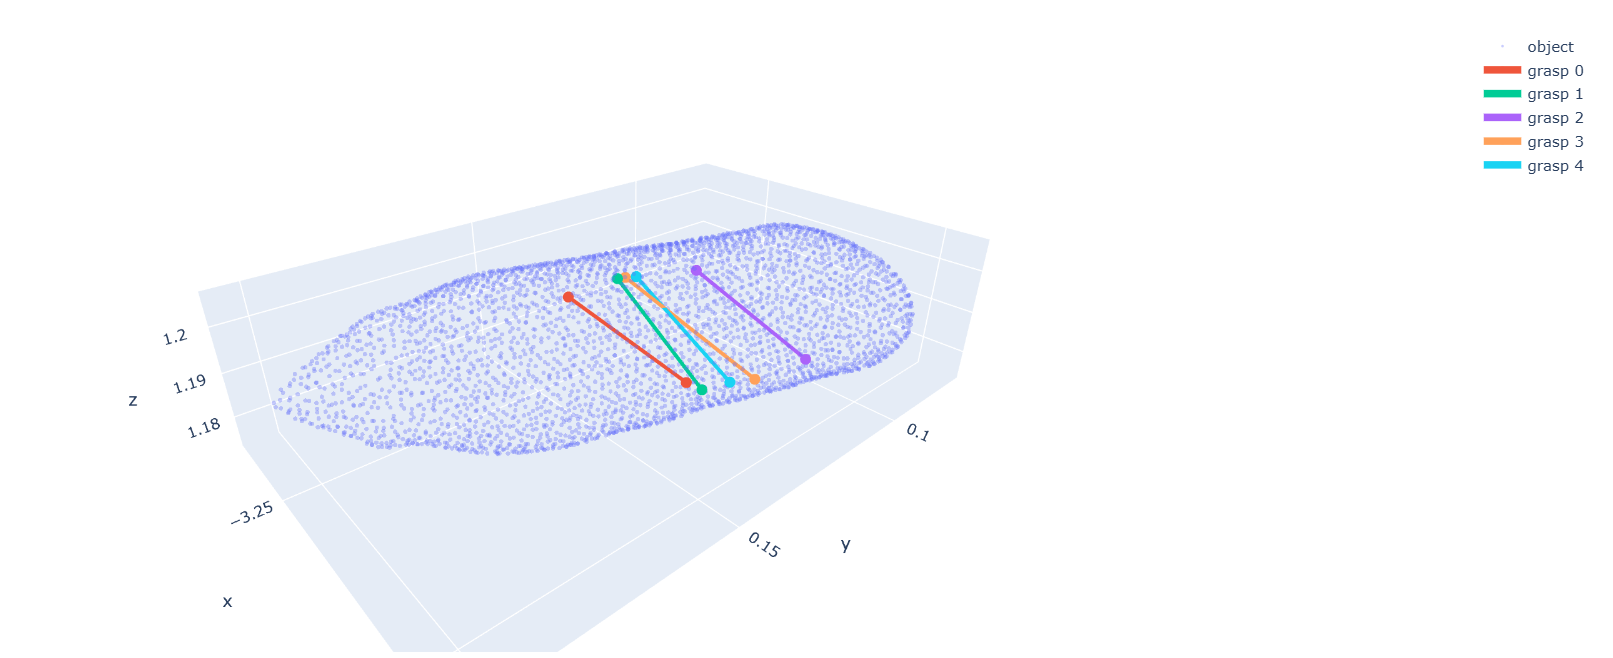
\includegraphics[width=\linewidth]{grasp_candidates.png}
\caption{Top-ranked antipodal grasp candidates generated on the reconstructed object point cloud. Candidate pairs are filtered using geometric constraints and later ranked using the proposed heuristic scoring framework.}
\label{fig:grasp_candidates}
\end{figure}

Instead of selecting grasps solely based on centroid proximity, the final system uses a weighted heuristic scoring framework that combines multiple geometric and physical criteria. Each grasp candidate is evaluated using antipodal quality, normal-axis alignment, grasp width consistency, PCA-based object alignment, self-clearance, scene-clearance, and floor-aware height reasoning to discourage grasps too close to the supporting surface.

PCA alignment encourages grasp directions aligned with the principal axes of the object geometry, particularly for elongated or anisotropic objects. However, geometric alignment alone is insufficient for reliable manipulation. Geometrically strong grasps may still be infeasible if the gripper collides with the object or nearby clutter during the approach motion. To address this problem, we introduce self-clearance and scene-clearance heuristics that evaluate whether the gripper approach corridor is obstructed by either the target object itself or the surrounding scene geometry.

The final grasp proposal is selected as the highest-scoring candidate and passed to the motion planning pipeline for execution.

\subsection{Grasp Evaluation}

To evaluate the contribution of each heuristic component, we performed a comparison study on several object types with different geometric properties, including regular box-like objects, irregular objects, and thin elongated objects. The evaluated configurations progressively enabled geometric scoring, PCA alignment, self-clearance reasoning, scene-clearance reasoning, and the complete weighted scoring framework. Table~\ref{tab:ablation} summarizes the main observations obtained from the experiments.

\begin{table}[!t]
\caption{Summary of the study observations across different object geometries.}
\label{tab:ablation}
\centering
\renewcommand{\arraystretch}{1.15}
\begin{tabular}{p{2.1cm} p{5.2cm}}
\toprule
Object & Main observation \\
\midrule
OreoBox & Baseline geometric scoring already produced feasible grasps, additional heuristics mainly improved robustness and grasp centrality. \\
\midrule
Lamp & PCA alignment improved geometric consistency, but PCA-only scoring could select blocked grasps. Self-clearance successfully removed infeasible candidates. \\
\midrule
Glue &  Elongated geometry experienced limitation. Clearance reduced heavily blocked candidates, but the full weighted scoring could still favor partially obstructed grasps. \\
\bottomrule
\end{tabular}
\end{table}

For regular box-like object such as OreoBox, the baseline geometric scoring already produced stable and physically feasible grasps. Additional heuristics mainly improved grasp centrality and robustness rather than drastically changing feasibility. In particular, the full system preferred grasps closer to the object center and farther from the floor region, leading to more stable grasp configurations.

For the lamp object, the effect of the heuristics became more visible. PCA-based scoring strongly improved alignment between the grasp direction and the object geometry. However, PCA-only scoring sometimes selected grasps that were blocked by the target geometry itself. Adding self-clearance reasoning successfully removed these infeasible candidates while still maintaining strong geometric alignment. This demonstrated that geometric consistency alone does not guarantee physical executability.

Elongated object such as the glue bottle was the third observed case. The baseline and PCA-only configurations frequently selected geometrically strong grasps that were partially blocked by the object geometry. Clearance reasoning substantially reduced the number of heavily blocked candidates, reducing the blocking count from 79 to 10 in the evaluated glue observations. However, the full weighted scoring could still occasionally favor highly aligned but partially obstructed grasps. This highlights a limitation of soft weighted scoring and suggests that future work may require stronger collision filtering or clearance parameters that adapt to different object geometries.

Overall, the study showed that geometric grasp quality alone is insufficient for robust manipulation in cluttered scenes. Clearance-aware reasoning substantially improved physical feasibility, particularly for irregular objects, while also revealing some limitations for elongated geometries.
\begin{thebibliography}{9}
\bibitem{sam2} N. Ravi \emph{et al.}, ``SAM~2: Segment Anything in
Images and Videos,'' \emph{arXiv:2408.00714}, 2024.
\bibitem{sam3} Meta AI, ``SAM~3: Segment Anything with Concepts,''
Technical Report, 2025.
\bibitem{clipseg} T. L\"uddecke and A. Ecker, ``Image Segmentation
Using Text and Image Prompts,'' in \emph{Proc. CVPR}, 2022.
\bibitem{dinov2} M. Oquab \emph{et al.}, ``DINOv2: Learning Robust
Visual Features without Supervision,'' \emph{arXiv:2304.07193}, 2023.
\end{thebibliography}

\end{document}
